\chapter{ADMM-IPC}\label{chap:my-work}

\section{基于惩罚力的流固耦合}

流固耦合作用力的公式\ref{eq:coupling-velocity}给出了流固耦合的基本力学原理。对于该约束,若采用拉格朗日视角的流体描述,即可转化为流体粒子无法穿透任何固体表面的约束。我们考虑用该约束来实现流体粒子与固体的相互耦合。由于固体常用三角网格来表示,因此本章主要考虑的碰撞即为流体与三角网格的耦合。对于一个三角面与流体粒子,其碰撞如图\ref{fig:coupling-example}所示。

\begin{figure}\centering
\tikzset{every picture/.style={line width=0.75pt}} %set default line width to 0.75pt        
\begin{tikzpicture}[x=0.75pt,y=0.75pt,yscale=-1,xscale=1]
%uncomment if require: \path (0,300); %set diagram left start at 0, and has height of 300

%Shape: Circle [id:dp6935007166126634] 
\draw  [fill={rgb, 255:red, 175; green, 86; blue, 86 }  ,fill opacity=1 ] (298,81.5) .. controls (298,77.91) and (300.91,75) .. (304.5,75) .. controls (308.09,75) and (311,77.91) .. (311,81.5) .. controls (311,85.09) and (308.09,88) .. (304.5,88) .. controls (300.91,88) and (298,85.09) .. (298,81.5) -- cycle ;
%Shape: Triangle [id:dp09215856226306518] 
\draw  [fill={rgb, 255:red, 74; green, 144; blue, 226 }  ,fill opacity=0.59 ] (446.43,80.57) -- (389.12,228.06) -- (228.44,134.69) -- cycle ;
%Straight Lines [id:da9852007763903861] 
\draw    (304.5,81.5) -- (332.06,133.23) ;
\draw [shift={(333,135)}, rotate = 241.96] [color={rgb, 255:red, 0; green, 0; blue, 0 }  ][line width=0.75]    (10.93,-3.29) .. controls (6.95,-1.4) and (3.31,-0.3) .. (0,0) .. controls (3.31,0.3) and (6.95,1.4) .. (10.93,3.29)   ;
%Straight Lines [id:da5006314821433624] 
\draw    (359,149) -- (355.09,57) ;
\draw [shift={(355,55)}, rotate = 87.56] [color={rgb, 255:red, 0; green, 0; blue, 0 }  ][line width=0.75]    (10.93,-3.29) .. controls (6.95,-1.4) and (3.31,-0.3) .. (0,0) .. controls (3.31,0.3) and (6.95,1.4) .. (10.93,3.29)   ;

% Text Node
\draw (231,73) node [anchor=north west][inner sep=0.75pt]   [align=left] {流体粒子};
% Text Node
\draw (289,92.4) node [anchor=north west][inner sep=0.75pt]    {$\mathbf{v}$};
% Text Node
\draw (313,160) node [anchor=north west][inner sep=0.75pt]   [align=left] {固体表面网格};
% Text Node
\draw (367,62.4) node [anchor=north west][inner sep=0.75pt]    {$\mathbf{n}$};
\end{tikzpicture}
\caption{基于碰撞的流固耦合示例:基于物理场的耦合被转化为流体粒子与固体表面网格的相互耦合。}\label{fig:coupling-example}
\end{figure}

尽管对于MPM流体而言,其不可压缩性是由速度场计算得到,但下一时间步的Advection步会按该速度场更新粒子位置,需要执行碰撞处理的位置指代的即为该更新后的目标位置。因此基于MPM法的流体迭代求解,可以也考虑其具有某个能量函数$E_f(\mathbf v_f)$,只不过该能量函数是由MPM求解器给出。从而,整个考虑了碰撞的隐式时间积分问题\ref{eq:impl-opt-of}可写作:
\begin{equation}
  \argmin{\mathbf x_s, \mathbf x_f} E_s(\mathbf x_s) + E_f(\mathbf v_f)\qquad s.t.\text{ no intersection}
\end{equation}
将IPC算法应用于该积分问题,则转化为如下的无约束的优化问题:
\begin{equation}\label{eq:ipc-fluid-base}
  \mathbf x_s, \mathbf v_f =  \argmin{\mathbf x_s, \mathbf v_f} E(\mathbf x_s, \mathbf v_f) + B(\mathbf x_s, \mathbf v_f)
\end{equation}
其中函数 $E(\mathbf x) = E_s(\mathbf x_s) + E_f(\mathbf v_f)$ 涵盖了所有动力学求解过程,例如流体不可压缩求解,布料和有限元的弹性动力学求解;函数 $B$ 涵盖了时间步的所有碰撞相关过程,例如原始IPC中处理的固体-固体碰撞,以及本文的流固耦合。

若直接对于问题\ref{eq:ipc-fluid-base}使用牛顿迭代法,即可得到以下基础算法:
\begin{algorithm}[H]
  \caption{IPC-流固耦合}\label{alg:ipc-fluid-base}
  \begin{algorithmic}[1]
    \label{algo:mpm-time-integration}
    \Require 系统各物体位置$\mathbf x^n$,速度$\mathbf v^n$,时间步长$h$
    \Ensure 积分结果 $\mathbf x^{n+1}, \mathbf v^{n+1}$
    \State $\mathbf x^{n+1}_{f} \leftarrow \mathrm{Advection} (\mathbf x^{n}_{f}, \mathbf v^{n}_f)$
    \State $k\leftarrow 0$
    \State $\mathbf x^{(k)} \leftarrow {\mathbf x^n_s, \mathbf v^n_f}$
    \While{未达到收敛条件}
      \State $\mathbf d \leftarrow -H^{-1} \nabla E(\mathbf x^{(k)}) + B(\mathbf x^{(k)})$
      \State 对 $\mathbf d$ 执行线搜索,确定系数$\alpha$
      \State $\mathbf x'\leftarrow \mathbf x + \alpha \mathbf d$
      \State 检查$\mathbf x^{(k)} \rightarrow \mathbf x'$碰撞情况,最小碰撞时间为 $ 0 < \alpha' \le 1$,更新 $\mathcal C$
      \State $\mathbf x^{(k+1)} \leftarrow \mathbf x^{(k)} + \alpha' \mathbf d$
      \State $k\leftarrow k + 1$ 
    \EndWhile
    \State ${\mathbf x^{n+1}_s, \mathbf v^{n+1}_f} \leftarrow\mathbf x^{(k-1)}$
    \State \Return $\mathbf x^{n+1}, \mathbf v^{n+1}$
  \end{algorithmic}
\end{algorithm}

\section{ADMM 解耦合}

与原先提到的IPC算法的缺点相同,算法\ref{alg:ipc-fluid-base}的第5步也存在需要反复计算$H^{-1}$,且保证正定的问题。观察到碰撞带来的约束相对是局部的,可对于问题\ref{eq:ipc-fluid-base}应用交替方向乘子法进行计算。对于碰撞约束,考虑其松弛变量为$\mathbf d$,则问题\ref{eq:ipc-fluid-base}可写为:
\begin{equation}
  \argmin{\mathbf x, \mathbf v} E(\mathbf{x}, \mathbf{v}) + B(\mathbf{d}) \quad s.t.D [\mathbf{x},\mathbf{v}]= \mathbf{d}
\end{equation}
其中矩阵$D$联系了$\mathbf{x, v, d}$。

在流体与网格物体耦合的过程中,主要考虑的是点-三角类型的碰撞处理。例如对于流体粒子 $\mathbf{f}\in \mathbb{R}^{3}$ 和三角网格点$\mathbf{x}_{0}, \mathbf{x}_{1}, \mathbf{x}_{2}$,流体粒子到三角面的法向的距离通过下式给出。
\begin{equation}
  \left|(\mathbf{f} - \mathbf{x}_{0})\cdot \frac{(\mathbf{x}_{1} - \mathbf{x}_{0})\times (\mathbf{x}_{2} - \mathbf{x}_{0})}{\|(\mathbf{x}_{1} - \mathbf{x}_{0})\times (\mathbf{x}_{2} - \mathbf{x}_{0})\|}\right|
\end{equation}
其中$\mathbf{d} = [\mathbf{f} ; \mathbf{x}_{0}; \mathbf{x}_{1}; \mathbf{x}_{2}],\quad \mathbf{f} = \mathbf x^{n} + h\mathbf v^{n+1}$。代入式\ref{eq:admm-algorithm},可得:
\begin{equation}
\begin{aligned}
\mathbf{x}^{(k)},\mathbf v^{(k)} &= \argmin{\mathbf{x}} F(\mathbf{x}^{(k)},\mathbf{v}^{(k)}, \mathbf{d}, \mathbf u^{(k-1)})\\
\mathbf{d}^{(k)}& = \argmin{\mathbf{d}} F(\mathbf{x}^{(k)},\mathbf{v}^{(k)}, \mathbf{d}, \mathbf u^{(k-1)})\\
\mathbf u^{(k)} &= \mathbf u^{(k-1)} + (D[\mathbf{x}^{(k)}, \mathbf v^{(k)}] - \mathbf{d}^{(k)})
\end{aligned}
\end{equation}

如果对于 $E$ 的解算也使用ADMM方法进行,且记 $\mathbf x = \mathbf x_s, \mathbf v_f$,则整个计算流程可以被简化为:

\begin{equation}
\begin{aligned}
\mathbf{x}^{(k)} &=\argmin{\mathbf{x}} I(\mathbf{x}) + \frac{1}{2} \| D_{z} \mathbf{x} - \mathbf{z}^{(k-1)} +\mathbf{u}_{z}^{(k-1)}\|_{W}^{2} +  \frac{\rho}{2} \| D_{d} \mathbf{x} - \mathbf{d}^{(k-1)} +\mathbf{u}_{d}^{(k-1)}\|_{2}^{2}\\
\mathbf{z}^{(k)} &= \arg\min_{\mathbf{z}} U(\mathbf{z}) + \frac{1}{2} \| D_{z} \mathbf{x}^{(k)} - \mathbf{z} + \mathbf{u}_{z}^{(k-1)}\|_{W}^{2}\\
\mathbf{u}_{z}^{(k)} &=\mathbf{u}_{z}^{(k-1)}+ (D_{z} \mathbf{x}^{(k)} - \mathbf{z}^{(k)})\\
\mathbf{d}^{(k)}&=\argmin{\mathbf{d}} B(\mathbf{d}) + \frac{\rho}{2} \| D_{d} \mathbf{x}^{(k)} - \mathbf{d} + \mathbf{u}_{d}\|_{2}^{2}\\
\mathbf{u}_{d}^{(k)}&=\mathbf{u}_{d}^{(k-1)} +\rho (D_{d} \mathbf{x}^{(k)} - \mathbf{d}^{(k)})
\end{aligned}
\end{equation}

对上述迭代,由于 $I(\mathbf{x})$ 对于固体求解为二次型,第1步可以使用Cholesky LLT分解进行加速求解;对流体求解为压强投影,可使用共轭梯度法进行快速求解。对于第2、4步,每一个单独的 $\mathbf{z}, \mathbf{d}$ 都可以进行并行计算。对于第3、5步,仅仅是简单的稀疏矩阵乘法和向量加法,可根据需要进行并行化处理。算法的第2、3步,是进行动力学解算,在第2章中已经进行介绍,更多的实现细节可见\ref{sec:experiment-admm}节。在本章主要关注整体算法的构造和碰撞求解(第4、5步)。

\section{碰撞解算}

所谓碰撞解算就是指 $\mathbf{d}$ 的解算。根据前文的分析,碰撞可能出现在任何出现位置更新的时刻,对于ADMM而言,即为第一步$\mathbf x$的更新需要进行碰撞解算。

\begin{figure}[hbt]
  \centering
\tikzset{every picture/.style={line width=0.75pt}} %set default line width to 0.75pt        

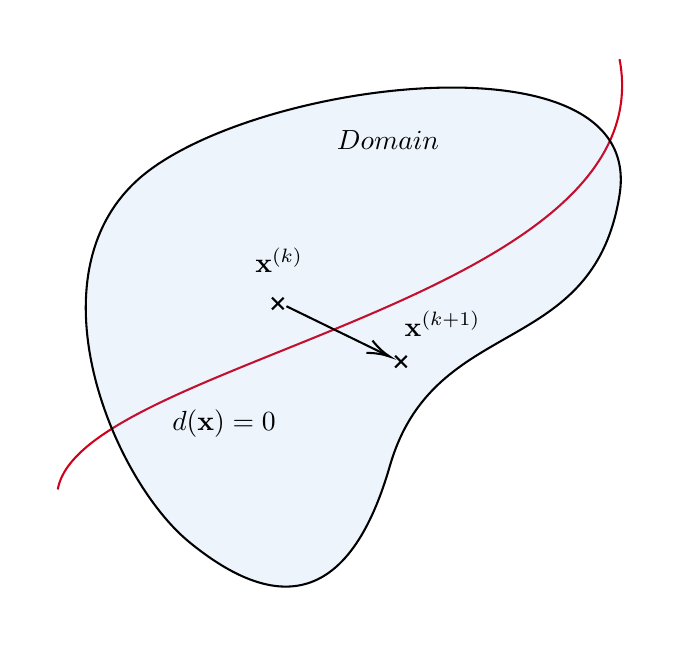
\begin{tikzpicture}[x=0.75pt,y=0.75pt,yscale=-1,xscale=1]
%uncomment if require: \path (0,310); %set diagram left start at 0, and has height of 310

%Curve Lines [id:da5390453303877039] 
\draw [color={rgb, 255:red, 208; green, 2; blue, 27 }  ,draw opacity=1 ]   (176.33,227.67) .. controls (187,165.67) and (469,137) .. (447,20.33) ;
%Shape: Polygon Curved [id:ds27867572621127656] 
\draw  [fill={rgb, 255:red, 74; green, 144; blue, 226 }  ,fill opacity=0.1 ] (215,78.33) .. controls (267.67,31) and (459.67,5.67) .. (447,85.67) .. controls (434.33,165.67) and (357.67,142.33) .. (336.33,216.33) .. controls (315,290.33) and (276.33,283) .. (239.67,253) .. controls (203,223) and (162.33,125.67) .. (215,78.33) -- cycle ;
\draw   (279.53,135.26) -- (285.14,140.86)(285.14,135.26) -- (279.53,140.86) ;
\draw   (338.86,163.26) -- (344.47,168.86)(344.47,163.26) -- (338.86,168.86) ;
%Straight Lines [id:da6123622539442625] 
\draw    (286.5,139.38) -- (334.54,162.79) ;
\draw [shift={(336.33,163.67)}, rotate = 205.99] [color={rgb, 255:red, 0; green, 0; blue, 0 }  ][line width=0.75]    (10.93,-3.29) .. controls (6.95,-1.4) and (3.31,-0.3) .. (0,0) .. controls (3.31,0.3) and (6.95,1.4) .. (10.93,3.29)   ;

% Text Node
\draw (270,109.73) node [anchor=north west][inner sep=0.75pt]    {$\mathbf{x}^{( k)}$};
% Text Node
\draw (342,140.4) node [anchor=north west][inner sep=0.75pt]    {$\mathbf{x}^{( k+1)}$};
% Text Node
\draw (230,187.73) node [anchor=north west][inner sep=0.75pt]    {$d(\mathbf{x}) =0$};
% Text Node
\draw (309.33,53.07) node [anchor=north west][inner sep=0.75pt]    {$Domain$};
\end{tikzpicture}
  \caption{迭代过程中碰撞的示意图:其中红色线表明$d = 0$,即发生了相交,也是内点法约束不能穿越的部分,蓝色部分表明可行域。}\label{fig:collision}
\end{figure}

如图\ref{fig:collision}所示,从$\mathbf x_n$到$\mathbf x_{n+1}$更新过程中,由于动力学解算的最小化问题中并不考虑碰撞,则可能穿越不可行区域,即发生了碰撞。如图\ref{fig:interpret-optimal}所示,假设 $\hat{\mathbf x} = \arg\min_{\mathbf{x}} I(\mathbf x) + \frac{1}{2}\|D_{z} \mathbf{x}-\mathbf{z} - \mathbf{u}_{z}\|_{W}^2$,从$\mathbf{x}$ 到$\hat{\mathbf{x}}$ 存在碰撞。

Lei 等人指出,对于IPC使用的障碍函数,其系数可以为$+\infty$。因此
\begin{equation}
  \mathbf{d}^{(k)}=\argmin{B(\mathbf d) = 0} \frac{\rho}{2} \| D_{d} \mathbf{x}^{(k)} - \mathbf{d} + \mathbf{u}_{d}\|_{2}^{2}
\end{equation}
其中的 $\mathbf d$ 还应满足无穿透条件,因此其最优解位置如图\ref{fig:interpret-optimal}所示。

\begin{figure}[hbt]
  \centering

\tikzset{every picture/.style={line width=0.75pt}} %set default line width to 0.75pt        

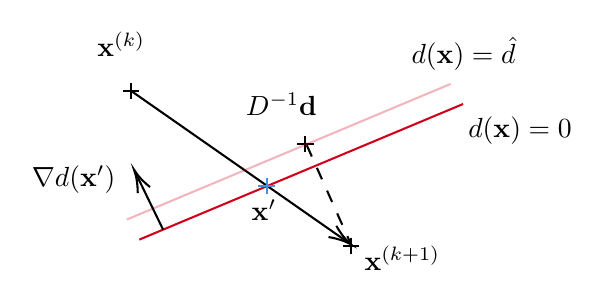
\begin{tikzpicture}[x=0.75pt,y=0.75pt,yscale=-1,xscale=1]
%uncomment if require: \path (0,300); %set diagram left start at 0, and has height of 300

\draw   (247.04,110.39) -- (254.96,110.39)(251,106.43) -- (251,114.36) ;
\draw   (353.04,185.06) -- (360.96,185.06)(357,181.1) -- (357,189.02) ;
%Straight Lines [id:da8691333295992784] 
\draw    (251,110.33) -- (355.36,183.19) ;
\draw [shift={(357,184.33)}, rotate = 214.92] [color={rgb, 255:red, 0; green, 0; blue, 0 }  ][line width=0.75]    (10.93,-3.29) .. controls (6.95,-1.4) and (3.31,-0.3) .. (0,0) .. controls (3.31,0.3) and (6.95,1.4) .. (10.93,3.29)   ;
%Straight Lines [id:da3846810796464156] 
\draw [color={rgb, 255:red, 208; green, 2; blue, 27 }  ,draw opacity=1 ]   (255,182) -- (411,116.67) ;
%Straight Lines [id:da34403059653345625] 
\draw  [dash pattern={on 4.5pt off 4.5pt}]  (335.67,136.5) -- (357,184.33) ;
\draw   (331.04,136.06) -- (338.96,136.06)(335,132.1) -- (335,140.02) ;
%Straight Lines [id:da7192719614800559] 
\draw [color={rgb, 255:red, 208; green, 2; blue, 27 }  ,draw opacity=0.29 ]   (249,172.33) -- (405,107) ;
%Straight Lines [id:da48171595095455455] 
\draw    (266.43,177.14) -- (253.3,150.09) ;
\draw [shift={(252.43,148.29)}, rotate = 64.12] [color={rgb, 255:red, 0; green, 0; blue, 0 }  ][line width=0.75]    (10.93,-3.29) .. controls (6.95,-1.4) and (3.31,-0.3) .. (0,0) .. controls (3.31,0.3) and (6.95,1.4) .. (10.93,3.29)   ;
\draw  [color={rgb, 255:red, 74; green, 144; blue, 226 }  ,draw opacity=1 ] (312.37,156.06) -- (320.3,156.06)(316.33,152.1) -- (316.33,160.02) ;

% Text Node
\draw (233.33,80.4) node [anchor=north west][inner sep=0.75pt]    {$\mathbf{x}^{( k)}$};
% Text Node
\draw (362,183.4) node [anchor=north west][inner sep=0.75pt]    {$\mathbf{x}^{( k+1)}$};
% Text Node
\draw (412,121.4) node [anchor=north west][inner sep=0.75pt]    {$d(\mathbf{x}) =0$};
% Text Node
\draw (304.83,109.73) node [anchor=north west][inner sep=0.75pt]    {$D^{-1}\mathbf{d}$};
% Text Node
\draw (384.67,83.07) node [anchor=north west][inner sep=0.75pt]    {$d(\mathbf{x}) =\hat{d}$};
% Text Node
\draw (201.71,144.83) node [anchor=north west][inner sep=0.75pt]    {$\nabla d(\mathbf{x} ')$};
% Text Node
\draw (307.67,161.07) node [anchor=north west][inner sep=0.75pt]    {$\mathbf{x} '$};


\end{tikzpicture}
\caption{计算$D^{-1}\mathbf d$:红色线为$d = 0$在$\mathbf x'$处的线性近似,$\nabla d(x')$为指向$\mathbf x^{(k)}$的法向。}\label{fig:interpret-optimal}
\end{figure}

为了加速其求解,将 $d(\mathbf x)$ 在碰撞处(即$d (\mathbf x')= 0$处)进行线性近似:
\begin{equation}
  d(\mathbf x) \approx (\nabla d(\mathbf x') )^T (\mathbf x  - \mathbf x')
\end{equation}
为使得$d = \hat d$,并利用距离函数$\|\nabla d\| \equiv 1$的性质,有
\begin{equation}
  D^{-1}\mathbf d = \mathbf x^{(k+1)} + (\hat d + (\nabla d(\mathbf x'))^T (\mathbf x' - \mathbf x^{(k+1)}))\nabla d(\mathbf x')
\end{equation}

另外,对于$k>1$时,第1步需要使用碰撞检测确定最大可行步长。令
\begin{equation}
  \tilde{\mathbf{x}}^{(k)}=\argmin{\mathbf{x}} I(\mathbf{x}) + \frac{1}{2} \| D_{z} \mathbf{x} - \mathbf{z}^{(k-1)} +\mathbf{u}_{z}^{(k-1)}\|_{W}^{2} +  \frac{1}{2} \| D_{d} \mathbf{x} - \mathbf{d}^{(k-1)} +\mathbf{u}_{d}^{(k-1)}\|_{2}^{2}
\end{equation}
以及 $t_{\min}=CCD(\mathbf{x}^{(k-1)}, \tilde {\mathbf{x}}^{(k)})$ 表示最近的碰撞时刻,则位置更新为:
\begin{equation}
  \mathbf x^{(k)} = t_{\min}\tilde{\mathbf x}^{(k)} + (1-t_{\min})\mathbf x^{(k - 1)}
\end{equation}
该算法利用每一步$\mathbf x^{(k)}\rightarrow \mathbf x^{(k+1)}$ 无碰撞来保证整个时间步内不发生穿透。而由于没有穿透发生,因此IPC在ADMM中的松弛变量$\mathbf u_d$ 恒为 0。

\section{算法描述}

总结以上内容,可得ADMM-IPC算法\ref{alg:ipc-fluid-final}。
\begin{algorithm}[H]
  \caption{ADMM-IPC}\label{alg:ipc-fluid-final}
  \begin{algorithmic}[1]
    \Require 系统各物体位置$\mathbf x^n$,速度$\mathbf v^n$,时间步长$h$
    \Ensure 积分结果 $\mathbf x^{n+1}, \mathbf v^{n+1}$
    \State $\mathbf x^{(1)} \leftarrow \mathbf [x^{n}, v^{n}], \mathbf u_z^{(0)} = \mathbf 0, k = 1$
    \While{not converged}
      \State $\mathbf z^{(k)} \leftarrow$ DynamicLocalStep()
      \State $\mathbf{u}_{z} ^{(k)} \leftarrow \mathbf{u}_{z}^{(k-1)} + (D_{z} \mathbf{x} ^{(k)}- \mathbf{z}^{(k)})$
      \State $\hat{\mathbf x}^{(k)} \leftarrow $DynamicGlobalStep()
      \State $\mathbf{d}^{(k)} \leftarrow \text{ContactLocalStep}(\mathbf{x}^{(k)}, \hat{\mathbf{x}}^{(k)})$
      \State $\hat{\mathbf{x}}^{(k)}\leftarrow \text{ContactGlobalStep}(\mathbf{d}^{(k)}, \hat{\mathbf{x}}^{(k)})$
      \State $t_I \leftarrow \text{CCD}(\mathbf x^{(k)}, \hat{\mathbf x}^{(k)})$
      \State $\mathbf{x}^{(k+1)} \leftarrow (1-t_{I}) \mathbf{x}^{(k)} +t_{I} \hat{\mathbf{x}}^{(k)}$
      \State $k \leftarrow k + 1$
    \EndWhile
  \end{algorithmic}
\end{algorithm}







